\documentclass[11pt,a4paper]{article}

\usepackage{../../templates/style}

\begin{document}

\begin{problem}{Mafia}{standard input}{standard output}{1 second}{64 megabytes}

พื้นที่แห่งหนึ่งมีกลุ่มมาเฟียที่มีอิทธิพลอยู่เป็นจำนวนมาก กำหนดให้ขอบเขตอิทธิพลของมาเฟียทุกกลุ่มมีลักษณะเป็นวงกลม โดยมาเฟียสองกลุ่มใดๆ สามารถมีขอบเขตอิทธิพลซ้อนทับกันบางส่วนหรือทั้งหมดหรือไม่ซ้อนทับกันเลยก็ได้ ทางรัฐบาลต้องการทำลายเขตอิทธิพลของมาเฟียเหล่านี้ให้ได้มากที่สุด จึงได้จัดตั้งตำรวจกองหนึ่งเพื่อคอยตรวจตราถนนสายต่างๆ ภายในเมือง แต่ทว่าวันนี้มีตำรวจเหลือเพียงนายเดียวเท่านั้น จึงต้องการให้คุณช่วยหาว่าตำรวจนายนี้จะเดินตรวจบนถนนสายใดเพื่อให้เดินผ่านเขตอิทธิพลให้ได้มากที่สุด โดยตำรวจจะเดินตรวจเป็นเส้นตรงที่ขนานแกน $x$ หรือแกน $y$ เท่านั้น และ\textbf{การเดินผ่านขอบเขตอิทธิพลหมายถึงการที่เส้นทางนั้นตัดผ่านขอบเขตอิทธิพลหรือสัมผัสวงกลมขอบเขตอิทธิพลก็ได้}

เมืองแห่งหนึ่งมีลักษณะเป็นสี่เหลี่ยมผืนผ้าขนาดกว้าง $N$ หน่วย ยาว $M$ หน่วย และมีกลุ่มมาเฟียที่มีอิทธิพลทั้งหมด $K$ กลุ่ม โดยแต่ละกลุ่มจะมีเขตอิทธิพลเป็นของตัวเองซึ่งอาจซ้อนทับกับกลุ่มอื่นได้ หน้าที่ของคุณคือหาถนนที่ดีที่สุดสำหรับตำรวจหนึ่งนายในการเดินตรวจตรา คือถนนดังกล่าวจะต้องผ่านเขตอิทธิพลของมาเฟียให้มากกลุ่มที่สุดเท่าที่จะทำได้

\bigskip
\underline{\textbf{โจทย์}}  จงเขียนโปรแกรมมเพื่อรับขนาดของเมืองและข้อมูลของกลุ่มมาเฟียทั้งหมด เพื่อคำนวนแล้วแสดงว่าจำนวนกลุ่มมาเฟียที่ตำรวจหนึ่งนายสามารถตรวจได้มากที่สุดเท่าที่เป็นไปได้คือเท่าไหร่ เมื่แเลือกที่จะตรวจบนถนนหนึ่งสายที่ขนานกับแกน $x$ หรือ $y$

\InputFile
\textbf{บรรทัดแรก} รับค่าจำนวนเต็ม $3$ จำนวนคือ $N$ $M$ $K$ ที่แทนขอบเขตของพื้นที่ทั้งหมด $(1 \leq N, M \leq 5\,000)$ และแทนจำนวนกลุ่มมาเฟียทั้งหมดที่มีภายในเมือง $(1 \leq K \leq 10\,000)$ ตามลำดับ

\textbf{บรรทัดที่ $2$ ถึง $K+1$} จะเป็นข้อมูลเขตอิทธิพลของมาเฟียแต่ละกลุ่ม โดยในบรรทัดที่ $i+1$ จะเป็นข้อมูลของมาเฟียกลุ่มที่ $i$ และในแต่ละบรรทัดจะรับจำนวนเต็มสามจำนวน $X$ $Y$ $R$ แทนค่าพิกัดตำแหน่งจุดศูนย์กลางของวงกลมอิทธิพล $(0 \leq X \leq N;  0 \leq Y \leq M)$  และรัศมีของวงกลม $(1 \leq R \leq 100)$ ตามลำดับ

\OutputFile

\textbf{มีบรรทัดเดียว} ที่แสดงจำนวนวงกลมที่ตัดได้มากที่สุด เมื่อลากเส้นขนานกับแกน $x$ หรือแกน $y$
\Examples

\begin{example}
\exmp{10 10 6
2 4 2
2 5 1
5 7 3
6 9 1
9 7 1
7 3 3}{5}%
\end{example}

\Note 

\begin{figure}[h]
\centering
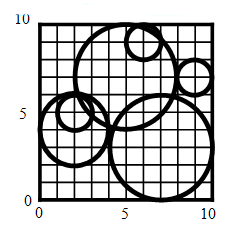
\includegraphics[width=0.5\textwidth]{../latex/img/1042/1042-1.png}
\end{figure}

จากตัวอย่างสามารถวาดวงกลมได้ดังรูป และเมื่อลากเส้นขนานแกน $x$
ที่ตำแหน่งความสูง $y = 6$ เส้นตรงนี้จะผ่านวงกลมทั้งหมด $5$ วง

\Source

การแข่งขันคณิตศาสตร์ วิทยาศาสตร์ โอลิมปิกแห่งประเทศไทย สาขาวิชาคอมพิวเตอร์ ประจำปี 2550

\end{problem}

\end{document}